\documentclass{article}
\usepackage{fullpage}
\usepackage{mathptmx}
\usepackage{graphicx}
\usepackage{amsmath}
\usepackage{floatflt}
\usepackage[aux]{rerunfilecheck}

\newcommand{\ds}{\displaystyle}

\title{MATH 110 Sample Final Exam 2 Solutions}
\author{Edward Doolittle}

\begin{document}
\maketitle

\begin{enumerate}
\item 
  \begin{enumerate}
  \item Write $y=x^{-3/2}-x^{2/3}+\sin x$ so
    $\ds \frac{dy}{dx} = (-3/2)x^{-5/2}-(2/3)x^{-1/3}+\cos x$.
  \item By the quotient rule,
    \begin{align*}
      \frac{dy}{dx} = \frac{\cos^2(x)\frac{d}{dx}\cos(x^2)
        - \cos(x^2)\frac{d}{dx}\cos^2(x)}{(\cos^2(x))^2}
      = \frac{\cos^2(x)\cdot -\sin(x^2)\cdot 2x
        - \cos(x^2) \cdot 2\cos(x) \cdot -\sin(x)}{\cos^4(x)}
    \end{align*}
    by the chain rule.
  \item Differentiating both sides,
    \begin{align*}
      \frac{d}{dx} (x+y+1)^{1/2} &= \frac{d}{dx} (1+x^2y^2)
      \\
      \frac{1}{2} (x+y+1)^{-1/2} \left(1 + \frac{dy}{dx}\right)
      &= 2xy^2 + x^2 2y\frac{dy}{dx}
    \end{align*}
    Solving for $dy/dx$,
    \begin{align*}
      (x+y+1)^{-1/2} + (x+y+1)^{-1/2} \frac{dy}{dx}
      &= 4xy^2 + 4x^2y \frac{dy}{dx}
      \\
      \left((x+y+1)^{-1/2} - 4x^2y\right) \frac{dy}{dx}
      &= 4xy^2 - (x+y+1)^{-1/2}
      \\
      \frac{dy}{dx}
      &= \frac{4xy^2-(x+y+1)^{-1/2}}{(x+y+1)^{-1/2}-4x^2y}
    \end{align*}
  \item By the Fundamental Theorem of Calculus,
    \begin{align*}
      \frac{dy}{dx} = \sqrt{\frac{x^2+1}{x^4+1}}
    \end{align*}
  \end{enumerate}
\item
  \begin{enumerate}
  \item Multiplying and dividing by $\pi$,
    \begin{align*}
      \lim_{x\to 0} \frac{\sin \pi x}{x}
      = \lim_{x\to 0} \frac{\sin \pi x}{\pi x} \cdot \pi
      = 1 \cdot \pi = \pi
    \end{align*}
    by the basic trig limit $\lim_{u\to 0} \sin u/u = 1$.
    (To be precise, you should use the rule $\lim_{x\to a} f(g(x))
    = f(\lim_{x\to a}g(x))$ with the continuous 
    functions $f(x)=\sin x/x$, $x\ne 0$, $f(0)=1$,
    and $g(x)=\pi x$, but it's OK if you don't go into
    full detail.)
  \item Multiplying out the denominator,
    \begin{align*}
      \lim_{x\to\infty} \frac{2x^3-7}{(1-x^2)(4x+7)}
      = \lim_{x\to\infty} \frac{2x^3-7}{-4x^3-7x^2+4x+7}
    \end{align*}
    Dividing through by the highest power of $x$ in the denominator,
    \begin{align*}
      \lim_{x\to\infty} \frac{2x^3-7}{-4x^3-7x^2+4x+7}
      = \lim_{x\to\infty} \frac{2-7/x^3}{-4-7/x+4/x^2+7/x^3}
      = \frac{2-0}{-4-0+0+0} = -\frac{1}{2}
    \end{align*}
  \item Note that the denominator vanishes at $x=-4$, and in fact so
    does the numerator, so we factor to obtain
    \begin{align*}
      \lim_{x\to -4} \frac{x^2+5x+4}{x^2+3x-4}
      = \lim_{x\to -4} \frac{(x+4)(x+1)}{(x+4)(x-1)}
      = \lim_{x\to -4} \frac{x+1}{x-1}
      = \frac{-4+1}{-4-1} = \frac{-3}{-5} = \frac{3}{5}
    \end{align*}
  \item Multiplying and dividing by the conjugate radical,
    \begin{align*}
      %\lim_{h\to 7} \frac{\sqrt{h+2}-3}{h-7} = 
      \lim_{h\to 7} \frac{\sqrt{h+2}-3}{h-7} 
      \frac{\sqrt{h+2}+3}{\sqrt{h+2}+3}
      = \lim_{h\to 7} \frac{(h+2)-9}{(h-7)(\sqrt{h+2}+3}
      = \lim_{h\to 7} \frac{1}{\sqrt{h+2}+3}
      = \frac{1}{\sqrt{7+2}+3} = \frac{1}{6}
    \end{align*}
  \end{enumerate}
\item 
  \begin{enumerate}
  \item Discontinuities occur at breaks in the graph, namely at $x=-1$
    and $x=2.5$.  (The arrows on the graph mean that the function continues
    smoothly to infinity on either side.)
  \item $f$ fails to be differentiable wherever it is not continuous, i.e.,
    at $x=-1$ and $x=2.5$, and also at points where it has a vertical
    tangent ($x=-3.5$) or a cusp ($x=4$) or an angle point (none on this
    graph).
  \end{enumerate}
\item Note that $f$ is continuous on $[1,2]$ (in fact, $f$ is continuous
  everywhere because it is a polynomial).  Furthermore, $f(1)=1^4+1-3=-1<0$
  and $f(2)=2^4+2-3=15>0$.  By the Intermediate Value Theorem, $f(x)$
  must equal $0$ somewhere between $x=1$ and $x=2$.
\item It is a good idea (although not necessary) to check that $(1,1)$ is
  a point on the curve: $1^2+1/(1\cdot 1) -1 = 1^2$, so it is.  
  Now by implicit differentiation,
  \begin{align*}
    \frac{d}{dx} \left( x^2 + (xy)^{-1} -1 \right)
    &= \frac{d}{dx} y^2
    \\
    2x - (xy)^{-2} \frac{d}{dx} (xy) &= 2y \frac{dy}{dx}
    \\
    2x - (xy)^{-2} \left(y + x\frac{dy}{dx}\right) &= 2y \frac{dy}{dx}
  \end{align*}
  You can solve for $dy/dx$ now, but it is easier to first substitute
  $(x,y)=(1,1)$ and then solve for $dy/dx$:
  \begin{align*}
    2-(1\cdot 1)^{-2} \left(1+1\frac{dy}{dx}\right) &= 2\cdot 1 \frac{dy}{dx}
    \\
    1-\frac{dy}{dx} &= 2\frac{dy}{dx}
    \\
    m = \frac{dy}{dx} &= \frac{1}{3}
  \end{align*}
  so the equation of the tangent line in point-slope form is
  \begin{align*}
    y-y_0 = m(x-x_0) \implies y-1 = \frac{1}{3} (x-1)
  \end{align*}
\item We have
  \begin{align*}
    V = \frac{4}{3} \pi r^3
  \end{align*}
  Differentiating with respect to $t$ (because this is a \textit{rates}
  problem),
  \begin{align*}
    \frac{dV}{dt} = 4 \pi r^2 \frac{dr}{dt}
  \end{align*}
  We are given that $dV/dt=0.3$ m$^3$/s and $r=2$ m, so
  \begin{align*}
    0.3 = 4\pi (2^2) \frac{dr}{dt}
    \implies \frac{dr}{dt} = \frac{3}{160\pi}
  \end{align*}
  The radius of the balloon is increasing at a rate of $3/(160\pi)$ m/s
  when the radius is $2$ m.
\item First, we need to calculate the derivatives of $f$ and factor them,
  if possible.  We have
  \begin{align*}
    f'(x) = 3x^2+6x-9=3(x^2+2x-3)=3(x+3)(x-1)
    \qquad
    f''(x) = 6x+6 = 6(x+1)
  \end{align*}
  \begin{enumerate}
  \item Critical point are where $f'(x)=0$ (at $x=-3$ and $x=1$) and where
    $f'(x)$ is undefined (nowhere).  The critical points split the line
    into three intervals $(-\infty,-3)$, $(-3,1)$, and $(1,\infty)$, and
    we determine the sign of $f'$ on each of those intervals as follows:
    \begin{center}
      \begin{tabular}{|c|c|c|c|}
        \hline
	$I$            & $x+3$ & $x-1$ & $f'(x)$ 
	\\
	\hline
	$(-\infty,-3)$ & $-$   & $-$   & $+$ 
	\\
	$(-3,1)$       & $+$   & $-$   & $-$
	\\
	$(1,\infty)$   & $+$   & $+$   & $+$
	\\
	\hline
      \end{tabular}
    \end{center}
    Since $f(x)$ increases to the left of $x=-3$ 
    and then decreases to the right of $x=-3$, $f$ has a local maximum at
    $x=-3$ by the first derivative test.  Similarly, since $f$ decreases
    to the left of $x=1$ and then increases to the right of $x=1$, $f$
    has a local minimum at $x=1$ by the first derivative test.

    Potential inflection points are where $f''(x)=0$ (at $x=-1$) and where
    $f''(x)$ is undefined (nowhere).  The potential inflection point 
    splits the $x$-axis into two intervals $(-\infty,-1)$ and $(-1,\infty)$,
    and we determine the sign of $f''$ on each of those intervals
    by a table like the following:
    \begin{center}
      \begin{tabular}{|c|c|c|}
        \hline
	$I$            & $x+1$ & $f''(x)$ 
	\\
	\hline
	$(-\infty,-1)$ & $-$   & $-$ 
	\\
	$(-1,\infty)$  & $+$   & $+$
	\\
	\hline
      \end{tabular}
    \end{center}
    (The table really isn't required for such a simple problem as this,
    but I include it for the sake of consistency.)  We see that $f$ is
    concave down to the left of $x=-1$ and concave up to the right of
    $x=-1$; since the concavity of $f$ changes at $x=-1$, it is an actual
    inflection point.

    Since $\lim_{x\to\infty} f(x)=\infty$ and $\lim_{x\to -\infty} f(x)
    = -\infty$, $f$ has no horizontal asymptotes.  Since $f$ does not
    blow up for any finite value of $x$, $f$ has no vertical asymptotes.
  \item We have already done all the work for this question in part (a).
    $f$ is increasing on intervals on which $f'(x)>0$, namely on the
    intervals $(-\infty,-3)$ and $(1,\infty)$, and $f$ is decreasing
    on the intervals on which $f'(x)<0$, namely on the interval $(-3,1)$.

    Similarly, $f$ is concave up on the intervals on which $f''(x)>0$,
    namely $(-1,\infty)$, and $f$ is concave down where $f''(x)<0$, namely
    $(-\infty,-1)$.
  \item To sketch the graph of $f$, we evaluate the $y$ values of the points
    of interest: the local max at $(-3,f(-3))=(-3,25)$, the local min at
    $(1,f(1))=(1,-7)$, and the inflection point at $(-1,f(-1))=(-1,9)$.
    We then plot those points on a graph and draw an increasing, concave
    down arc to the left of $(-3,25)$; a decreasing, concave down arc from 
    $(-3,25)$ to $(-1,9)$; a decreasing, concave up arc from $(-1,9)$ to
    $(1,-7)$; and an increasing, concave up arc to the right of $(1,-7)$.
    \begin{figure}[htbp]
      \begin{center}
        \includegraphics[width=5.5in]{sketch.eps}
      \end{center}
      \caption{The graph of $f(x)=x^3+3x^2-9x-2$}
      \label{fig:sketch}
    \end{figure}
    Your graph should look something like the graph in Figure~\ref{fig:sketch}.
  \end{enumerate}
\item See Figure~\ref{fig:flower}.
  \begin{figure}[htbp]
    \begin{center}
      \includegraphics[width=2in]{flower.eps}
    \end{center}
    \caption{Diagram for the flower garden problem}
    \label{fig:flower}
  \end{figure}
  The constraint for this problem is $xy=12$, and the objective to be
  minimized is the cost of the fence, $C=3y+2x+3y=2x+6y$.  Eliminating
  $y=12/x$ from the objective gives $C(x)=2x+6(12/x)=2x+72/x$.  Differentiating
  gives $C'(x)=2-72/x^2$ with critical points at $x=-6$, $x=0$ (both of which
  are outside the domain of $C$; we can assume $x>0$) and $x=6$.  We
  can write $C'(x)=2(x+6)(x-6)/x^2$ from which it follows that $C'(x)<0$ on
  the interval $(0,6)$ and $C'(x)>0$ on $(6,\infty)$, so $C(x)$ has a global
  minimum at $x=6$.  In summary, the dimensions of the $12$ m$^2$
  garden that minimizes the cost of the fence are $x=6$ m (the side facing
  the house is $6$ m in length) and $y=2$ m 
  (the sides that are touching the house are $2$ m in length).
\item First we sketch the region between the curves.  See Figure~\ref{fig:area}.
  \begin{figure}[htbp]
    \begin{center}
      \includegraphics[width=4in]{area.eps}
    \end{center}
    \caption{The region bounded by $y=x^2-2x$ and $y=x$}
    \label{fig:area}
  \end{figure}
  The intersection points are given by $x^2-2x=y=x$ or $x^2-2x=x$ or $x^2-3x=0$
  or $x=0,3$.  (Since there are only two intersection points, that confirms
  the assumption implicit in the diagram that there is only one bounded
  region defined by the two curves.)  The area is
  \begin{align*}
    A = \int_0^3 (f(x)-g(x)) \; dx
    = \int_0^3 (x - (x^2-2x)) \; dx
    = \int_0^3 (3x-x^2) \; dx
    = \left. \vphantom{\int} \frac{3}{2} x^2 - \frac{1}{3} x^3 \right|_0^3
    = \left(\frac{27}{2} - 9\right) - (0-0)
    = \frac{9}{2}
  \end{align*}
\item 
  \begin{enumerate}
  \item Making the substitution $u=1+x^2$, $du=2x\; dx$, $du/2=x \; dx$,
    \begin{align*}
      \int x \; \sin(1+x^2) \; dx
      = \int \sin u \frac{du}{2}
      = \frac{1}{2} (-\cos u) + C
      = -\frac{1}{2} \cos(1+x^2) + C
    \end{align*}
    You should check by differentiating.
  \item Expanding the integrand,
    \begin{align*}
      \int \left(\frac{1}{x} + \sqrt{x} \right)^2 \; dx
      = \int \left(\frac{1}{x^2} + 2\frac{1}{x} \sqrt{x} + x\right) \; dx
      = \int (x^{-2} + 2 x^{-1/2} + x) \; dx
      = \frac{x^{-3}}{-3} + 2 \frac{x^{1/2}}{1/2} + \frac{x^2}{2} + C
    \end{align*}
    Strictly speaking, since the integrand is discontinuous at $x=0$,
    we should write the answer as
    \begin{align*}
      F(x) = \begin{cases}
        -x^{-3}/3+4x^{1/2}+x^2/2 + C_1, &\mbox{$x<0$} \\
	-x^{-3}/3+4x^{1/2}+x^2/2 + C_2, &\mbox{$0<x$,}
      \end{cases}
    \end{align*}
    but the first answer is adequate.
  \item \textbf{Solution 1.} We first find the indefinite integral and
    then evaluate the definite integral.
    Let $u=\pi/x$, and then $du = -\pi/x^2 \; dx$, $-du/\pi=dx/x^2$, and
    we have 
    \begin{align*}
      \int \frac{1}{x^2} \; \cos\left(\frac{\pi}{x}\right) \; dx
      = -\frac{1}{\pi} \int \cos u \; du
      = -\frac{1}{\pi} \sin u + C
      = -\frac{1}{\pi} \sin\left(\frac{\pi}{x}\right) + C
    \end{align*}
    You should check the result by differentiating.  Now, evaluating the
    definite integral,
    \begin{align*}
      \int_1^2 \frac{1}{x^2} \; \cos\left(\frac{\pi}{x}\right) \; dx
      = \left. \vphantom{\int} -\frac{1}{\pi} \sin\left(\frac{\pi}{x}\right)
      \right|_1^2
      = -\frac{1}{\pi} \sin\left(\frac{\pi}{2}\right)
      + \frac{1}{\pi} \sin\left(\frac{\pi}{1}\right)
      = -\frac{1}{\pi} 1 + \frac{1}{\pi} 0
      = -\frac{1}{\pi}
    \end{align*}

    \textbf{Solution 2.}  We can do the above in a single step.  As before,
    let $u=\pi/x$.  Then $-du/\pi=dx/x^2$, but we also note $x=1$ implies
    $u=\pi$ and $x=2$ implies $u=\pi/2$, and we have
    \begin{align*}
      \int_1^2 \frac{1}{x^2} \cos\left(\frac{\pi}{x}\right) \; dx
      = -\frac{1}{\pi} \int_{\pi}^{\pi/2} \cos u \; du
      = \left. -\frac{1}{\pi} \sin u \right|_{\pi}^{\pi/2}
      = -\frac{1}{\pi} \sin(pi/2)+\frac{1}{\pi} \sin(\pi)
      = -\frac{1}{\pi}
    \end{align*}
    Note that the limits of integration go from right to left rather
    than from left to right.  There's nothing wrong with that; just remember
    that $\int_a^b f(x) \; dx = -\int_b^a f(x) \; dx$.
  \item As above, there are two ways to evaluate this integral.  Let's do
    it the fast way.  Let $u=3x+16$.  Then $du=3\; dx$; $du/3=dx$; 
    when $x=0$, $u=16$; and when $x=3$, $u=25$.  So we have
    \begin{align*}
      \int_0^3 \sqrt{3x+16} \; dx
      = \int_{16}^{25} u^{1/2} \frac{du}{3}
      = \left. \frac{1}{3} \frac{2}{3} u^{3/2} \right|_{16}^{25}
      = \frac{2}{9} (5^3-4^3)
      = \frac{122}{9} 
    \end{align*}
    I suggest you check the answer by trying it the other way.
  \end{enumerate}
\end{enumerate}

\end{document}

